\subsection{Überblick}
DYCOS (\underline{DY}namic \underline{C}lassification 
algorithm with c\underline{O}ntent and \underline{S}tructure) ist ein 
Knotenklassifizierungsalgorithmus, der Ursprünglich in \cite{aggarwal2011} vorgestellt 
wurde. Er klassifiziert einzelne Knoten, indem $r$ Random Walks der Länge $l$,
startend bei dem zu klassifizierenden Knoten $v$ gemacht werden. Dabei
werden die Labels der besuchten Knoten gezählt. Das Label, das am häufigsten
vorgekommen ist, wird als Label für $v$ gewählt.
DYCOS nutzt also die sog. Homophilie, d.~h. die Eigenschaft, dass
Knoten, die nur wenige Hops von einander entfernt sind, häufig auch
ähnlich sind \cite{bhagat}. Der DYCOS-Algorithmus nimmt jedoch nicht 
einfach den Graphen für dieses Verfahren, sondern erweitert ihn mit 
Hilfe der zur Verfügung stehenden Texte.\\
Für diese Erweiterung wird zuerst wird Vokabular $W_t$ bestimmt, das 
charakteristisch für eine Knotengruppe ist. Wie das gemacht werden kann
und warum nicht einfach jedes Wort in das Vokabular aufgenommen wird,
wird in \cref{sec:vokabularbestimmung} erläutert.\\
Nach der Bestimmung des Vokabulars wird für 
jedes Wort im Vokabular ein Wortknoten zum Graphen hinzugefügt. Alle
Knoten, die der Graph zuvor hatte, werden nun \enquote{Strukturknoten}
genannt.
Ein Strukturknoten $v$ wird genau dann mit einem Wortknoten $w \in W_t$
verbunden, wenn $w$ in einem Text von $v$ vorkommt.
Der DYCOS-Algorithmus betrachtet also die Texte, die einem Knoten 
zugeordnet sind, als eine Multimenge von Wörtern. Das heißt, zum einen 
wird nicht auf die Reihenfolge der Wörter geachtet, zum anderen wird 
bei Texten eines Knotens nicht zwischen verschiedenen 
Texten unterschieden. Jedoch wird die Anzahl der Vorkommen 
jedes Wortes berücksichtigt.

\begin{figure}[htp]
    \centering
    \tikzstyle{vertex}=[draw,black,circle,minimum size=10pt,inner sep=0pt]
\tikzstyle{edge}=[very thick]
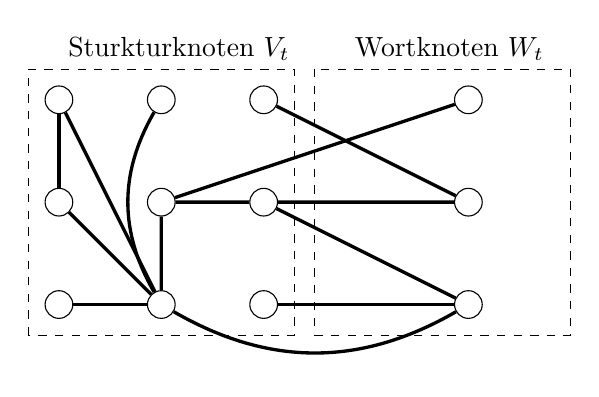
\begin{tikzpicture}[scale=1.3]
    \node (a)[vertex] at (0,0) {};
    \node (b)[vertex]  at (0,1) {};
    \node (c)[vertex] at (0,2) {};
    \node (d)[vertex] at (1,0) {};
    \node (e)[vertex]  at (1,1) {};
    \node (f)[vertex] at (1,2) {};
    \node (g)[vertex] at (2,0) {};
    \node (h)[vertex] at (2,1) {};
    \node (i)[vertex] at (2,2) {};

    \node (x)[vertex] at (4,0) {};
    \node (y)[vertex] at (4,1) {};
    \node (z)[vertex] at (4,2) {};

    \draw[edge] (a) -- (d);
    \draw[edge] (b) -- (d);
    \draw[edge] (b) -- (c);
    \draw[edge] (c) -- (d);
    \draw[edge] (d) -- (e);
    \draw[edge] (d) edge[bend left] (f);
    \draw[edge] (d) edge[bend right] (x);
    \draw[edge] (g) edge (x);
    \draw[edge] (h) edge (x);
    \draw[edge] (h) edge (y);
    \draw[edge] (h) edge (e);
    \draw[edge] (e) edge (z);
    \draw[edge] (i) edge (y);

    \draw [dashed] (-0.3,-0.3) rectangle (2.3,2.3);
    \draw [dashed] (2.5,2.3) rectangle (5, -0.3);

    \node (struktur)[label={[label distance=0cm]0:Sturkturknoten $V_t$}] at (-0.1,2.5) {};
    \node (struktur)[label={[label distance=0cm]0:Wortknoten $W_t$}] at (2.7,2.5) {};
\end{tikzpicture}

    \caption{Erweiterter Graph}
    \label{fig:erweiterter-graph}
\end{figure}

Entsprechend werden zwei unterschiedliche Sprungtypen unterschieden,
die strukturellen Sprünge und inhaltliche Mehrfachsprünge:

\begin{definition}
    Sei $G_{E,t} = (V_t, E_{S,t} \cup E_{W,t}, V_{L,t}, W_{t})$ der
    um die Wortknoten $W_{t}$ erweiterte Graph.

    Dann heißt das zufällige wechseln des aktuell betrachteten
    Knoten $v \in V_t$ zu einem benachbartem Knoten $w \in V_t$
    ein \textbf{struktureller Sprung}.
\end{definition}
\goodbreak
Im Gegensatz dazu benutzten inhaltliche Mehrfachsprünge
tatsächlich die Grapherweiterung:
\begin{definition}
    Sei $G_t = (V_t, E_{S,t} \cup E_{W,t}, V_{L,t}, W_{t})$ der
    um die Wortknoten $W_{t}$ erweiterte Graph.

    Dann heißt das zufällige wechseln des aktuell betrachteten
    Knoten $v \in V_t$ zu einem benachbartem Knoten $w \in W_t$
    und weiter zu einem zufälligem Nachbar $v' \in V_t$ von $w$
    ein \textbf{inhaltlicher Mehrfachsprung}.
\end{definition}

Jeder inhaltliche Mehrfachsprung beginnt und endet also in einem Strukturknoten,
springt über einen Wortknoten und ist ein Pfad der Länge~2.

Ob in einem Sprung der Random Walks ein struktureller Sprung oder
ein inhaltlicher Mehrfachsprung gemacht wird, wird jedes mal zufällig
neu entschieden. Dafür wird der Parameter $0 \leq p_S \leq 1$ für den Algorithmus 
gewählt. Mit einer Wahrscheinlichkeit von $p_S$ wird eine struktureller
Sprung durchgeführt und mit einer Wahrscheinlichkeit
von $(1-p_S)$ ein modifizierter inhaltlicher Mehrfachsprung, wie er in
\cref{sec:sprungtypen} erklärt wird, gemacht. Dieser 
Parameter gibt an, wie wichtig die Struktur des Graphen im Verhältnis
zu den textuellen Inhalten ist. Bei $p_S = 0$ werden ausschließlich
die Texte betrachtet, bei $p_S = 1$ ausschließlich die Struktur des
Graphen.

Die Vokabularbestimmung kann zu jedem Zeitpunkt $t$ durchgeführt 
werden, muss es aber nicht.

In \cref{alg:DYCOS} wird der DYCOS-Algorithmus als 
Pseudocode vorgestellt.

\begin{algorithm}
    \begin{algorithmic}[1]
        \Require \\$G_{E,t} = (V_t, E_{S,t} \cup E_{W,t}, V_{L,t}, W_t)$ (Erweiterter Graph),\\
                 $r$ (Anzahl der Random Walks),\\
                 $l$ (Länge eines Random Walks),\\
                 $p_s$ (Wahrscheinlichkeit eines strukturellen Sprungs),\\
                 $q$ (Anzahl der betrachteten Knoten in der Clusteranalyse)
        \Ensure  Klassifikation von $V_t \setminus V_{L,t}$\\
        \\

        \ForAll{Knoten $v$ in $V_t \setminus V_{L,t}$}
            \State $d \gets $ defaultdict
            \For{$i$ von $1$ bis $r$}
                \State $w \gets v$
                \For{$j$ von $1$ bis $l$}
                    \State $sprungTyp \gets \Call{random}{0, 1}$
                    \If{$sprungTyp \leq p_S$}
                        \State $w \gets$ \Call{SturkturellerSprung}{$w$}
                    \Else
                        \State $w \gets$ \Call{InhaltlicherMehrfachsprung}{$w$}
                    \EndIf
                    \State $w \gets v.\Call{GetLabel}{ }$ \Comment{Zähle das Label}
                    \State $d[w] \gets d[w] + 1$
                \EndFor
            \EndFor

            \If{$d$ ist leer} \Comment{Es wurde kein gelabelter Knoten gesehen}
                \State $M_H \gets \Call{HäufigsteLabelImGraph}{ }$
            \Else
                \State $M_H \gets \Call{max}{d}$
            \EndIf
            \\
            \State \Comment{Wähle aus der Menge der häufigsten Label $M_H$ zufällig eines aus}
            \State $label \gets \Call{Random}{M_H}$ 
            \State $v.\Call{AddLabel}{label}$ \Comment{und weise dieses $v$ zu}
        \EndFor
        \State \Return Labels für $V_t \setminus V_{L,t}$
    \end{algorithmic}
\caption{DYCOS-Algorithmus}
\label{alg:DYCOS}
\end{algorithm}

\subsection{Datenstrukturen}
Zusätzlich zu dem gerichteten Graphen $G_t = (V_t, E_t, V_{L,t})$ 
verwaltet der DYCOS-Algorithmus zwei weitere Datenstrukturen:
\begin{itemize}
    \item Für jeden Knoten $v \in V_t$ werden die vorkommenden Wörter,
          die auch im Vokabular $W_t$ sind,
          und deren Anzahl gespeichert. Das könnte z.~B. über ein 
          assoziatives Array geschehen. Wörter, die nicht in 
          Texten von $v$ vorkommen, sind nicht im Array. Für
          alle vorkommenden Wörter ist der gespeicherte Wert zum 
          Schlüssel \enquote{Wort} die Anzahl der Vorkommen von 
          \enquote{Wort} in den Texten von $v$.
    \item Für jedes Wort des Vokabulars $W_t$ wird eine Liste von 
          Knoten verwaltet, in deren Texten das Wort vorkommt.
    \item An einigen Stellen macht ein assoziatives Array, auch 
          \enquote{dictionary} oder \enquote{map} genannt, Sinn.
          Zustätzlich ist es nützlich, wenn diese Datenstruktur für 
          unbekannte Schlüssel keinen Fehler ausgibt, sondern für diese
          Schlüssel den Wert 0 annimmt. Eine solche Datenstruktur
          wird in Python \texttt{defaultdict} genannt und ich werde
          im Folgenden diese Benennung beibehalten.
\end{itemize}

\subsection{Sprungtypen}\label{sec:sprungtypen}
Die beiden bereits definierten Sprungtypen, der strukturelle Sprung
sowie der inhaltliche Mehrfachsprung werden im folgenden erklärt.
\goodbreak
Der strukturelle Sprung entspricht einer zufälligen Wahl eines 
Nachbarknotens, wie es in \cref{alg:DYCOS-structural-hop}
gezeigt wird.
\begin{algorithm}[H]
    \begin{algorithmic}[1]
        \Procedure{SturkturellerSprung}{Knoten $v$, Anzahl $q$}
            \State $n \gets v.\Call{NeighborCount}{}$ \Comment{Wähle aus der Liste der Nachbarknoten}
            \State $r \gets \Call{RandomInt}{0, n-1}$ \Comment{einen zufällig aus}
            \State $v \gets v.\Call{Next}{r}$ \Comment{Gehe zu diesem Knoten}
            \State \Return $v$
        \EndProcedure
    \end{algorithmic}
\caption{Struktureller Sprung}
\label{alg:DYCOS-structural-hop}
\end{algorithm}

Bei inhaltlichen Mehrfachsprüngen ist jedoch nicht sinnvoll so direkt
nach der Definition vorzugehen,  also
direkt von einem strukturellem Knoten 
$v \in V_t$ zu einem mit $v$ verbundenen Wortknoten $w \in W_t$ zu springen
und von diesem wieder zu einem verbundenem strutkurellem Knoten 
$v' \in V_t$. Würde man dies machen, wäre zu befürchten, dass
aufgrund von Homonymen die Qualität der Klassifizierung verringert
wird. So hat \enquote{Brücke} im Deutschen viele Bedeutungen.
Gemeint sein können z.~B. das Bauwerk, das Entwurfsmuster der
objektorientierten Programmierung oder ein Teil des Gehirns.

Deshalb wird für jeden Knoten $v$, von dem aus man einen inhaltlichen
Mehrfachsprung machen will folgendes Clusteranalyse durchgeführt:
\begin{enumerate}[label=C\arabic*),ref=C\arabic*]
    \item[C1] Gehe alle in $v$ startenden Random Walks der Länge 2 durch
          und erstelle eine Liste $L$, der erreichbaren Knoten $v'$. Speichere
          außerdem, durch wie viele Pfade diese Knoten $v'$ jeweils erreichbar sind.
    \item[C2] Betrachte im folgenden nur die Top-$q$ Knoten, wobei $q \in \mathbb{N}$
          eine zu wählende Konstante des Algorithmus ist. \label{list:aggregate.2}
    \item[C3] Wähle mit Wahrscheinlichkeit $\frac{\Call{Anzahl}{v'}}{\sum_{w \in L} \Call{Anzahl}{v'}}$
          den Knoten $v'$ als Ziel des Mehrfachsprungs.
\end{enumerate}

Konkret könnte also ein Inhaltlicher Mehrfachsprung sowie wie in
\cref{alg:DYCOS-content-multihop} beschrieben umgesetz werden.

\begin{algorithm}
  \caption{Inhaltlicher Mehrfachsprung}
  \label{alg:DYCOS-content-multihop}
    \begin{algorithmic}[1]
        \Procedure{InhaltlicherMehrfachsprung}{Knoten $v$}
            \State \textit{//Alle Knoten bestimmen, die von $v$ aus über Pfade der Länge 2 erreichbar sind}
            \State \textit{//Zusätzlich wird für diese Knoten die Anzahl der Pfade der Länge 2 bestimmt,}
            \State \textit{//durch die sie erreichbar sind}
            \State $reachableNodes \gets$ defaultdict
            \ForAll{Wortknoten $w$ in $v.\Call{getWordNodes}{ }$}
                \ForAll{Strukturknoten $x$ in $w.\Call{getStructuralNodes}{ }$}
                    \State $reachableNodes[x] \gets reachableNodes[x] + 1$
                \EndFor
            \EndFor

            \State \textit{//Im folgenden wird davon ausgegangen, dass man über Indizes wahlfrei auf}
            \State \textit{//Elemente aus $M_H$ zugreifen kann. Dies muss bei der konkreten Wahl}
            \State \textit{//der Datenstruktur berücksichtigt werden.}
            \State $M_H \gets \Call{max}{reachableNodes, q}$ \Comment{Also: $|M_H| = q$, falls $|reachableNodes|\geq q$}
            \State \textit{//Generate dictionary with relative frequencies}
            \State $s \gets 0$
            \ForAll{Knoten $x$ in $M_H$}
                \State $s \gets s + reachableNodes[x]$
            \EndFor
            \State $relativeFrequency \gets $ Dictionary
            \ForAll{Knoten $x$ in $M_H$}
                \State $relativeFrequency \gets \frac{reachableNodes[x]}{s}$
            \EndFor
            \State \textit{//Wähle Knoten $i$ mit einer Wahrscheinlichkeit entsprechend seiner relativen}
            \State \textit{//Häufigkeit an Pfaden der Länge 2}
            \State $random \gets \Call{random}{0, 1}$
            \State $r \gets 0.0$
            \State $i \gets 0$
            \While{$s < random$}
                \State $r \gets r + relativeFrequency[i]$
                \State $i \gets i + 1$
            \EndWhile
            
            \State $v \gets M_H[i-1]$ 
            \State \Return $v$
        \EndProcedure
    \end{algorithmic}
\end{algorithm}

\subsection{Vokabularbestimmung}\label{sec:vokabularbestimmung}
Da die Größe des Vokabulars die Datenmenge signifikant beeinflusst,
liegt es in unserem Interesse so wenig Wörter wie möglich ins
Vokabular aufzunehmen. Insbesondere sind Wörter nicht von Interesse,
die in fast allen Texten vorkommen, wie im Deutschen z.~B.
\enquote{und}, \enquote{mit} und die Pronomen. Es ist wünschenswert
Wörter zu wählen, die die Texte möglichst stark voneinander Unterscheiden.
Der DYCOS-Algorithmus wählt die Top-$m$ dieser Wörter als Vokabular,
wobei $m \in \mathbb{N}$ eine Festzulegende Konstante ist. In \cite[S. 365]{aggarwal2011}
wird der Einfluss von $m \in \Set{5,10, 15,20}$ auf die Klassifikationsgüte
untersucht und festgestellt, dass die Klassifikationsgüte mit größerem
$m$ sinkt, sie also für $m=5$ für den DBLP-Datensatz am höchsten ist.
Für den CORA-Datensatz wurde mit $m \in \set{3,4,5,6}$ getestet und 
kein signifikanter Unterschied festgestellt.

Nun kann man manuell eine Liste von zu beachtenden Wörtern erstellen
oder mit Hilfe des Gini-Koeffizienten automatisch ein Vokabular erstellen.
Der Gini-Koeffizient ist ein statistisches Maß, das die Ungleichverteilung
bewertet. Er ist immer im Intervall $[0,1]$, wobei $0$ einer 
Gleichverteilung entspricht und $1$ der größtmöglichen Ungleichverteilung.

Sei nun $n_i(w)$ die Häufigkeit des Wortes $w$ in allen Texten mit 
der $i$-ten Knotenbeschriftung.
\begin{align}
    p_i(w) &:= \frac{n_i(w)}{\sum_{j=1}^{|\L_t|} n_j(w)} &\text{(Relative Häufigkeit des Wortes $w$)}\\
    G(w)   &:= \sum_{j=1}^{|\L_t|} p_j(w)^2              &\text{(Gini-Koeffizient von $w$)}
\end{align}
In diesem Fall ist $G(w)=0$ nicht möglich, da zur Vokabularbestimmung
nur Wörter betrachtet werden, die auch vorkommen.

Ein Vorschlag, wie die Vokabularbestimmung implementiert werden kann,
ist als Pseudocode mit \cref{alg:vokabularbestimmung}
gegeben. Dieser Algorithmus benötigt neben dem Speicher für den
Graphen, die Texte sowie die $m$ Vokabeln noch $\mathcal{O}(|\text{Verschiedene Wörter in } S_t| \cdot (|\L_t| + 1))$
Speicher. Die Average-Case Zeitkomplexität beträgt 
$\mathcal{O}(|\text{Wörter in } S_t|)$, wobei dazu die Vereinigung
von Mengen $M,N$ in $\mathcal{O}(\min{|M|, |N|})$ sein muss.

\begin{algorithm}
    \begin{algorithmic}[1]
        \Require \\
                 $V_{L,t}$ (beschriftete Knoten),\\
                 $\L_t$ (Beschriftungen),\\
                 $f:V_{L,t} \rightarrow \L_t$ (Beschriftungsfunktion),\\
                 $m$ (Gewünschte Vokabulargröße)
        \Ensure  $\M_t$ (Vokabular)\\

        \State $S_t \gets \Call{Sample}{V_{L,t}}$ \Comment{Wähle eine Teilmenge $S_t \subseteq V_{L,t}$ aus}
        \State $\M_t \gets \bigcup_{v \in S_t} \Call{getTextAsSet}{v}$ \Comment{Menge aller Wörter}
        \State $cLabelWords \gets (|\L_t|+1) \times |\M_t|$-Array, mit 0en initialisiert\\

        \ForAll{$v \in V_{L,t}$} \Comment{Gehe jeden Text Wort für Wort durch}
            \State $i \gets \Call{getLabel}{v}$
            \ForAll{$(word, occurences) \in \Call{getTextAsMultiset}{v}$}
                \State $cLabelWords[i][word] \gets cLabelWords[i][word] + occurences$
                \State $cLabelWords[i][|\L_t|] \gets cLabelWords[i][|\L_t|] + occurences$
            \EndFor
        \EndFor
        \\
        \ForAll{Wort $w \in \M_t$}
            \State $p \gets $ Array aus $|\L_t|$ Zahlen in $[0, 1]$
            \ForAll{Label $i \in \L_t$}
                \State $p[i] \gets \frac{cLabelWords[i][w]}{cLabelWords[i][|\L_t|]}$
            \EndFor

            \State $w$.gini $\gets 0$
            \ForAll{$i \in 1, \dots, |\L_t|$}
                \State $w$.gini $\gets$ $w$.gini + $p[i]^2$
            \EndFor
        \EndFor

        \State $\M_t \gets \Call{SortDescendingByGini}{\M_t}$
        \State \Return $\Call{Top}{\M_t, m}$
    \end{algorithmic}
\caption{Vokabularbestimmung}
\label{alg:vokabularbestimmung}
\end{algorithm}

Die Menge $S_t$ kann aus der Menge aller Dokumente, deren 
Knoten beschriftet sind, mithilfe des in \cite{Vitter} vorgestellten
Algorithmus bestimmt werden.

